\documentclass[11pt,a4paper]{article}

\usepackage[T1]{fontenc}
\usepackage[utf8]{inputenc}
\usepackage[ngerman]{babel}
\usepackage{lmodern}
\usepackage[a4paper,margin=2.5cm]{geometry}
\usepackage{microtype}
\usepackage{parskip}
\usepackage{csquotes}
\usepackage{enumitem}
\usepackage{graphicx}
\usepackage{tabularx}
\usepackage{wrapfig}
\usepackage[hidelinks]{hyperref}

\setlist[enumerate]{leftmargin=*,label=\arabic*.}

\title{Anfrage zur Filmvorf\"uhrung von \enquote{Die Kommissarin} im Kino International\\mit Gespr\"ach am 19.~April~2026}
\author{}
\date{}

\begin{document}

\maketitle
\vspace{-0.95cm}
\noindent
\begin{minipage}[t]{0.70\textwidth}
\footnotesize Hiermit m\"ochten wir anfragen, ob das Kino International am 19.~April~2026 bereit w\"are, eine Filmvorf\"uhrung mit anschlie{\ss}endem Gespr\"ach auszurichten. Die Veranstaltung wird vom \href{https://eles-studienwerk.de/}{Ernst Ludwig Ehrlich Studienwerk (ELES)} im Rahmen der Abendveranstaltungsreihe \href{https://gemeinsam-gegen-antisemitismus.de/}{\enquote{Nie wieder!? Gemeinsam gegen Antisemitismus \& f\"ur eine plurale Gesellschaft}} organisiert. Sie richtet sich an die Stipendiat:innen des Ernst Ludwig Ehrlich Studienwerks sowie an die \"Offentlichkeit; die Veranstaltung ist als kostenfreies Angebot mit Voranmeldung angedacht.
\end{minipage}\hfill
\begin{minipage}[t]{0.25\textwidth}
\footnotesize
\vspace{-0.1cm}
\raggedleft
\href{https://gemeinsam-gegen-antisemitismus.de/}{
\includegraphics[width=\linewidth,height=4.4\baselineskip,keepaspectratio]{NW_Logo_quer2_inverted.png}}
\end{minipage}
\vspace{-0.2cm}

\section*{Der Film und sein historischer Kontext}

\begin{wrapfigure}[12]{r}{0.24\textwidth}
  \vspace{-1.1\baselineskip}
  \centering
  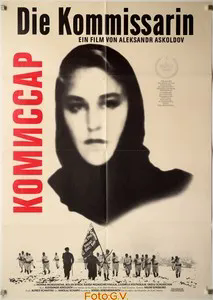
\includegraphics[width=\linewidth]{Kommissarin_plakat.png}
\end{wrapfigure}

Aleksandr Askoldovs Film \enquote{Die Kommissarin} entstand 1967 nach Wassili Grossmans Erz\"ahlung \enquote{In der Stadt Berdytschiw}. Berdytschiw erscheint darin als j\"udisch gepr\"agter Raum des ehemaligen Zarenreichs, in dem Revolution, B\"urgerkrieg und Alltag ineinandergreifen. Im Zentrum steht die schwangere Kommissarin Klawdija Wawilowa, die bei einer armen j\"udischen Familie unterkommt. So verschiebt der Film den Blick von der politischen Gro{\ss}geschichte auf N\"ahe, Verletzlichkeit und existenzielle Unsicherheit.

Askoldov zeigt Geschichte nicht heroisch, sondern als Raum von Gewalt, Abh\"angigkeit und moralischer Desorientierung. Historische Dramatik, Groteske und traumartige Bilder verdichten diese Erfahrung zu einer br\"uchigen, bedrohlichen Landschaft.

Zugleich r\"uckt der Film eine j\"udisch-sowjetische Erfahrungswelt ins Zentrum, die im sowjetischen Kino meist marginal blieb. Im Pogrom kulminieren B\"urgerkriegsgewalt, antisemitische Deutungsmuster wie der Mythos der sogenannten \enquote{\.Zydokomuna} (\enquote{Jewish Bolshevism}) und der sp\"atere Schatten der Shoah. Gerade deshalb wurde \enquote{Die Kommissarin} verboten und erst w\"ahrend der Glasnost \"offentlich gezeigt. Heute gilt der Film als Schl\"usselwerk, weil er die Verbindung von B\"urgerkrieg, Pogromgewalt und j\"udisch-sowjetischer Erinnerung sichtbar macht.

\section*{Kurzkonzeption}

Das Ernst Ludwig Ehrlich Studienwerk organisiert anl\"asslich von 80 Jahren Kriegsende eine Filmveranstaltung, die Film und Gespr\"ach miteinander verbindet. Gezeigt wird Aleksandr Askoldovs \enquote{Die Kommissarin} (1967), ein bedeutender sowjetischer Film \"uber j\"udische Erfahrungen w\"ahrend des B\"urgerkriegs, der wegen seiner Darstellung von Pogromgewalt und j\"udischer Verletzlichkeit fast zwanzig Jahre lang von der sowjetischen Zensur verboten war. Anschlie{\ss}end diskutieren Prof.\ Dr.\ Irina Scherbakowa, Mitbegr\"underin der mit dem Friedensnobelpreis ausgezeichneten Menschenrechtsorganisation MEMORIAL, und Prof.\ Dr.\ Viktoriya Sukovata, Gastwissenschaftlerin am Dubnow-Institut Leipzig und Expertin f\"ur Holocaustdarstellungen im sowjetischen und postsowjetischen Film, \"uber Film, j\"udisch-sowjetische Geschichte und Erinnerungskultur.

Die Veranstaltung nimmt das Datum des Kriegsendes nicht nur als historischen Anlass, sondern auch als Ausgangspunkt f\"ur die Frage, welche Erfahrungen in staatlich gepr\"agten Erinnerungskulturen sichtbar werden und welche verdr\"angt bleiben. \enquote{Die Kommissarin} ist daf\"ur besonders geeignet, weil der Film keine heroische Siegeserz\"ahlung reproduziert, sondern Schutzlosigkeit, famili\"are Solidarit\"at und historische Bedrohung in den Mittelpunkt r\"uckt.

\section*{Warum Kino International}

Unser Programm Kino Kaddish (mehr Informationen unter \url{https://kino-kaddish.org}) zielt darauf ab, Film und Ort bewusst miteinander zu verbinden. Vor diesem Hintergrund sehen wir in einer Veranstaltung im Kino International, gerade im Zuge seiner Wiederer\"offnung, eine besondere Gelegenheit. Als architektonisch und filmhistorisch bedeutender Ort der DDR-Kinokultur bietet es einen passenden Rahmen, um Filmkunst aus dem \"ostlichen kulturellen Raum neu sichtbar zu machen. Zugleich erlaubt der Ort, die komplexe Geschichte dieser Filmkultur mitzudenken, die sowohl bemerkenswerte k\"unstlerische Arbeiten hervorgebracht hat als auch von Fragen der Zensur, Ideologie und kulturellen Identit\"at gepr\"agt war.

Gerade f\"ur \enquote{Die Kommissarin} ist dieser Zusammenhang produktiv: Der Film steht selbst f\"ur eine gro{\ss}e k\"unstlerische Form, die im sowjetischen Kontext unterdr\"uckt wurde und erst versp\"atet \"offentlich zirkulieren konnte. Eine Vorf\"uhrung im Kino International w\"urde daher nicht nur einen thematisch passenden Auff\"uhrungsort bieten, sondern auch einen Raum er\"offnen, in dem \"uber Sichtbarkeit, politische Rahmung und die Nachgeschichte des osteurop\"aischen Kinos nachgedacht werden kann. Im Rahmen der Wiederer\"offnung lie{\ss}e sich so ein Programm realisieren, das die Geschichte des Hauses ernst nimmt und zugleich neue Perspektiven auf j\"udisch-sowjetische Erfahrung und Erinnerungskultur \"offnet.

\section*{Gespr\"achspartnerinnen}

\textbf{\href{https://www.zfl-berlin.org/person/scherbakowa.html}{Prof.\ Dr.\ Irina Scherbakowa}} ist Germanistin, Historikerin und Mitbegr\"underin der Menschenrechtsorganisation \href{https://www.memorial.de/}{MEMORIAL}. Ihre Arbeit zu m\"undlicher Geschichte, Stalinismus und sowjetischer Erinnerungspolitik zeigt, wie der staatliche \enquote{Siegesmythos} unbequeme Erinnerungen systematisch verdr\"angte. F\"ur das Gespr\"ach bringt sie die Frage mit, warum ein Film wie \enquote{Die Kommissarin}, der j\"udische Verletzlichkeit statt revolution\"aren Heroismus zeigt, zwanzig Jahre lang unzeigbar war und was seine versp\"atete Sichtbarkeit \"uber sowjetische und postsowjetische Geschichtspolitik verr\"at.

\textbf{\href{https://www.dubnow.de/person/prof-dr-victoryia-a-sukovata}{Prof.\ Dr.\ Viktoriya Sukovata}} war an der Universit\"at Charkiw t\"atig und forscht derzeit als Gastwissenschaftlerin am Dubnow-Institut Leipzig. Ihre Arbeiten untersuchen, wie der Holocaust im sowjetischen und postsowjetischen Film dargestellt, verschl\"usselt oder unsichtbar gemacht wurde. Sie zeigt, dass j\"udisches Leid in der sowjetischen Kultur meist unter allgemeinen Kategorien wie \enquote{sowjetische Zivilisten} aufgel\"ost und antisemitische Gewalt selten eigens benannt wurde. Ihr Blick auf \enquote{Die Kommissarin} sch\"arft die Frage, was es bedeutet, dass Askoldov Berdytschiw als ausdr\"ucklich j\"udischen Raum inszeniert und die Pogromgewalt beim Namen nennt.

Gemeinsam er\"offnen beide Perspektiven einen Dialog \"uber die politischen und kulturellen Bedingungen, unter denen Erinnerung entsteht, unterdr\"uckt und wiedergewonnen wird.

\section*{Vorschlag f\"ur den Ablauf}

\noindent\textbf{Sonntag, 19.~April~2026}

\small
\renewcommand{\arraystretch}{1.08}
\begin{tabularx}{\textwidth}{@{}p{3.1cm}X@{}}
\textbf{Zeit} & \textbf{Programmpunkt} \\
17:30--18:00 & \textbf{Einlass und Begr\"u{\ss}ung}\\
& Ankommen, kurze Einf\"uhrung in das Programm und den Anlass des Abends. \\
18:00--19:44 & \textbf{Filmvorf\"uhrung}\\
& Aleksandr Askoldovs \enquote{Die Kommissarin} (104 Min.). \\
19:45--20:35 & \textbf{Podiumsgespr\"ach mit Irina Scherbakowa und Viktoriya Sukovata (angefragt)}\\
& Diskussion \"uber Film, j\"udisch-sowjetische Erfahrung, Pogromgewalt, Shoah und Erinnerungskultur. \\
20:35--21:00 & \textbf{Offener Ausklang}\\
& Fragen, Austausch und Vernetzung; der Ablauf ist selbstverst\"andlich flexibel und kann an die Disposition des Hauses angepasst werden. \\
\end{tabularx}

\end{document}
